%!TEX TS-program = xelatex
\documentclass[]{friggeri-cv}
\usepackage{afterpage}
\usepackage{hyperref}
\usepackage{color}
\usepackage{xcolor}
\hypersetup{
    pdftitle={},
    pdfauthor={},
    pdfsubject={},
    pdfkeywords={},
    colorlinks=false,       % no lik border color
   allbordercolors=white    % white border color for all
}
\addbibresource{bibliography.bib}
\RequirePackage{xcolor}
\definecolor{pblue}{HTML}{0395DE}

\begin{document}
\header{Yi}{~Cao}
{\href{mailto:ycao2@binghamton.edu}{ycao2@binghamton.edu} | 347-238-5686 |
33-46 84 ST, Jackson Heights, NY, 11372}
% Fake text to add separator
%\fcolorbox{white}{gray}{\parbox{\dimexpr\textwidth-2\fboxsep-2\fboxrule}{.....}}

% In the aside, each new line forces a line break
\hfill
\begin{aside}
	\section{Education}
		\textbf{M.A. Biological Sciences\\May 2015}
		{Binghamton University, State University of New York}
		\textbf{B.S., Biotechnology\\June 2009}
		{Fudan University}
		\section{Skills}
		\textbullet{Python}
		\textbullet{Mathematica}
		\textbullet{Microsoft Office}
		\textbullet{Genetic Biology}
		\textbullet{Cellular Biology}
		\textbullet{Bioinformatics}
		\textbullet{Animal Experiments}
		\textbullet{Protein Biochemistry}
		\textbullet{Photoshop}
		\textbullet{Agile Management}

  \section{Languages}
    \textbf{English}
\includegraphics[scale=0.40]{img/5stars.png}
    \textbf{Mandrian}
\includegraphics[scale=0.40]{img/5stars.png}
    \textbf{Cantonese}
\includegraphics[scale=0.40]{img/4stars.png}
    \textbf{French}
\includegraphics[scale=0.40]{img/2stars.png}
  %\section{Personal Skills}
  %  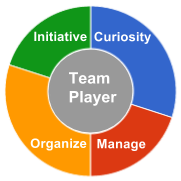
\includegraphics[scale=0.62]{img/personal.png}
  %  ~
\end{aside}
\section{Experience}
\begin{entrylist}

  \entry
    {04/09-07/09}
    {Development Assistant}
		{Genesky Bio-Tech Co, Ltd., Shanghai, China}
		{
			\begin{tightemize}
				\item{Built up T-vector cloning platform, performed PCR with genomic DNA isolated
					from clinical samples.}
				\item{Analyzed genotypes according to sequencing results and composed the report
					sent to clients, like academic labs and clinics.}
			\end{tightemize}
		}

  \entry
    {07/08-08/08}
		{Summer Research Intership}
    {China Novartis Institues for BioMedical Research}
		{
			\begin{tightemize}
				\item{Identified and isolated mutant cancer cell gene targets and determined
					receptor function by transient transfection.}
				\item{Assisted nude mice model experiments.}
			\end{tightemize}
		}

    \entry
    {07/12-09/12}
		{Hospital Volunteer}
		{Lourdes Hospital, Binghamton, NY}
    {
			\begin{tightemize}
				\item{Served in emergency room and hospital.}
				\item{Familiarized with procedures in emergency room, from greeting
					to financing.}
				\item{Assisted nurses, and helped patients and visitors to solve non-treatment
					issues.}
				\item{Maintained supplies, including food, beverage, linens, disposable medical
					supplies.}
			\end{tightemize}
		}

    \entry
    {01/10-05/12}
		{Teaching Assistant}
		{Biology Department, SUNY Binghamton}
    {
			\begin{tightemize}
				\item{Prepared experiments materials, designed and taught lab sections,
					demonstrated techniques.}
				\item{Held weekly office hours, graded all associated materials.}
				\item{Guided students' group research project and evaluated
					presentation.}
				\item{Demonstrated proficiency at computer aided teaching and research tools and
					the web search engines.}
			\end{tightemize}
		}

\end{entrylist}

\section{Projects}
\begin{entrylist}
	\entry
		{09/14-03/14}
		{Master paper project: opioid receptor signaling and its role in cancer
			progression}
		{}
		{
			\begin{tightemize}
				\item{Discussed conflicting research findings by studying more than 50 BioMedical
					literatures.}
			\end{tightemize}
		}
	\entry
		{02/12-05/12}
		{Business Plan of Biomedical Start-up Company}
		{}
		{
			\begin{tightemize}
				\item{Created a business plan for biomedical start-up FyreSaw
					Rhythm, which develops an innovative cardiac device to treat atrial
					fibrillation by surgery.}
				\item{Worked in a team in creative thinking on the idea.}
				\item{Composed the business model, exit strategy, and financials
					sections of the business plan.}
			\end{tightemize}
		}
	\entry
		{02/11-05/11}
		{Dynamic modeling of PI3K/Akt signaling induced by mu opioid receptor}
		{}
		{
			\begin{tightemize}
				\item{Obtained protein immunoblots data from my independent laboratory project
					conducted on human cancer cells, and applied it for the configuration of
					modeling.}
				\item{Designed and graphed a dynamic Model in Mathematica, simulating activity
					status and expression of multiple messenger molecules involved in this
					signaling process.}
			\end{tightemize}
		}
	\entry
		{09/09-01/10}
		{Data mining of microarray database in search of biomarker candidates}
		{}
		{
			\begin{tightemize}
				\item{Designed a Python program used to search GSO database for cancer
					biomarkers, potentially leading to metastasis of breast cancer, prostate
					cancer, and lung cancer.}
				\item{Presented the primary outcome in annual Binghamton University biology
					department seminar.}
			\end{tightemize}
		}
\end{entrylist}

\end{document}
